\renewcommand{\theequation}{\theenumi}
\begin{enumerate}[label=\arabic*.,ref=\thesubsection.\theenumi]
\numberwithin{equation}{enumi}
\item given that $\to$
\\friquency of no with unit digit 6 = 14
\\
probability of unit digit to be 6 = P(X=6)
\\
\begin{align} 
P\left(X=6\right) &= \frac{14}{200}
\\
&= 0.07
\end{align}
codes for the above equation can be get from here
\begin{lstlisting}
codes/probexm/probexm4.py
\end{lstlisting}
\begin{figure}[!ht]
	\centering
	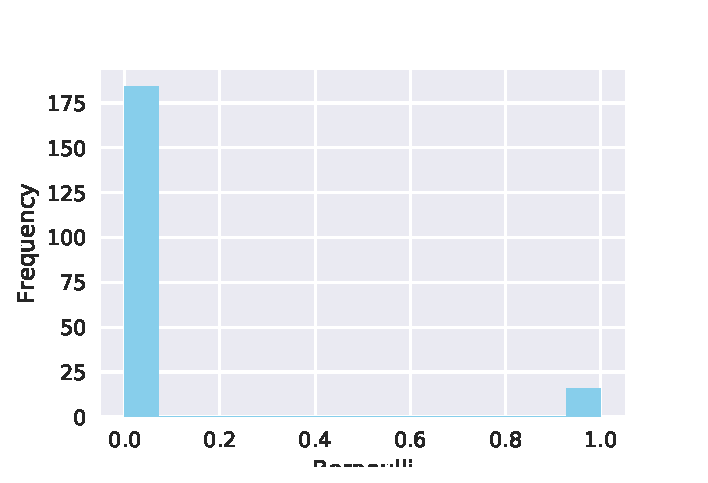
\includegraphics[width=\columnwidth]{./figures/probexm/probexm4.eps}
	\caption{bernoulli distribution of no to be 6}
	\label{fig:bt2}
	\begin{lstlisting}
	figs/probexm/probexm4.eps
	\end{lstlisting}
\end{figure}
\end{enumerate}